\documentclass{article}
\usepackage[utf8]{inputenc}
\usepackage{graphicx}


\begin{document}
\section{Comparison Table}

\hspace{-3cm}
\resizebox{18cm}{!}{
\begin{tabular}{|l r r r r| r r r r r r | r r|}
\hline
Benchmark & $|V|$ & Vars & Clauses & Solutions & $n$ & Calls & Samples & valid & $t_q (\mu s)$ & $t_q* (\mu s)$ & Samples & $t_u/t_q$ \\
\hline
blasted\_case47 & 28.0 & 118.0 & 328.0 & 262144.0 & 267.0 & 7235.0 & 10006004.0 & 0.607 & 7.3 & 16.5 & 882827.0 & 514.0 \\
\hline
blasted\_case110 & 17.0 & 287.0 & 1263.0 & 16384.0 & 1440.0 & 23042.0 & 10000186.0 & 0.835 & 23.4 & 23.9 & 3033041.0 & 46.0 \\
\hline
s820a\_7\_4 & 23.0 & 616.0 & 1703.0 & 591872.0 & 143.0 & 3455.0 & 10005763.0 & 0.809 & 6.9 & 28.0 & 626538.0 & 759.0 \\
\hline
s820a\_15\_7 & 23.0 & 685.0 & 1987.0 & 722944.0 & 128.0 & 3094.0 & 10000853.0 & 0.727 & 7.8 & 45.5 & 495836.0 & 850.0 \\
\hline
s1238a\_3\_2 & 32.0 & 686.0 & 1850.0 & 2466250752.0 & 9.0 & 328.0 & 10116002.0 & 0.915 & 3.4 & 200.2 & 16302.0 & 59275.0 \\
\hline
s1196a\_3\_2 & 32.0 & 690.0 & 1805.0 & 1038090240.0 & 11.0 & 386.0 & 10007402.0 & 0.826 & 3.8 & 207.3 & 22110.0 & 39257.0 \\
\hline
s832a\_15\_7 & 23.0 & 693.0 & 2017.0 & 3713024.0 & 85.0 & 2063.0 & 10008371.0 & 0.813 & 5.6 & 86.8 & 122276.0 & 4834.0 \\
\hline
blasted\_case\_1\_b12\_2 & 45.0 & 827.0 & 2725.0 & 274877906944.0 & 2.0 & 121.0 & 10039060.0 & 0.823 & 4.5 & 260.8 & 19899.0 & 36762.0 \\
\hline
blasted\_squaring16 & 72.0 & 1627.0 & 5835.0 & 1.86527593088e+12 & 0.0 & 61.0 & 10671382.0 & 0.25 & 19.4 & 1265.0 & 1463.0 & 116830.0 \\
\hline
blasted\_squaring7 & 72.0 & 1628.0 & 5837.0 & 274408144896.0 & 3.0 & 250.0 & 10122013.0 & 0.623 & 8.5 & 731.5 & 6116.0 & 63478.0 \\
\hline
70.sk\_3\_40 & 40.0 & 4670.0 & 15864.0 & 8589934592.0 & 8.0 & 304.0 & 10134785.0 & 0.365 & 15.8 & 1220.6 & 8360.0 & 24979.0 \\
\hline
ProcessBean.sk\_8\_64 & 64.0 & 4768.0 & 14458.0 & nan & 1.0 & 98.0 & 10081716.0 & 0.371 & 12.7 & 1238.2 & 7524.0 & 34611.0 \\
\hline
56.sk\_6\_38 & 38.0 & 4842.0 & 17828.0 & 3690987520.0 & 10.0 & 336.0 & 10148125.0 & 0.519 & 9.3 & 808.8 & 9383.0 & 37908.0 \\
\hline
35.sk\_3\_52 & 52.0 & 4915.0 & 10547.0 & 4.3980465111e+12 & 2.0 & 95.0 & 10717156.0 & 1.0 & 3.8 & 279.1 & 7612.0 & 115962.0 \\
\hline
80.sk\_2\_48 & 48.0 & 4969.0 & 17060.0 & 1.09951162778e+12 & 2.0 & 126.0 & 10252598.0 & 0.325 & 13.8 & 1336.3 & 5478.0 & 43694.0 \\
\hline
7.sk\_4\_50 & 50.0 & 6683.0 & 24816.0 & 2.19902325555e+12 & 2.0 & 124.0 & 10139607.0 & 0.216 & 23.6 & 1788.5 & 4136.0 & 41648.0 \\
\hline
doublyLinkedList.sk\_8\_37 & 37.0 & 6890.0 & 26918.0 & 2038431744.0 & 116.0 & 3748.0 & 10016007.0 & 0.038 & 2751.5 & 6050.2 & 0.0 & 0.0 \\
\hline
19.sk\_3\_48 & 48.0 & 6993.0 & 23867.0 & 2.95980289229e+12 & 1.0 & 90.0 & 10291254.0 & 0.208 & 21.8 & 1846.9 & 2343.0 & 64524.0 \\
\hline
29.sk\_3\_45 & 45.0 & 8866.0 & 31557.0 & 347892350976.0 & 2.0 & 113.0 & 10000333.0 & 0.132 & 44.6 & 2634.6 & 1012.0 & 108459.0 \\
\hline
isolateRightmost.sk\_7\_481 & 481.0 & 10057.0 & 35275.0 & nan & 0.0 & 59.0 & 10412010.0 & 0.188 & 54.6 & 2734.1 & 0.0 & 0.0 \\
\hline
17.sk\_3\_45 & 45.0 & 10090.0 & 27056.0 & 274877906944.0 & 3.0 & 157.0 & 10181716.0 & 0.192 & 29.1 & 2046.2 & 275.0 & 413272.0 \\
\hline
81.sk\_5\_51 & 51.0 & 10775.0 & 38006.0 & 1.81419418583e+13 & 1.0 & 52.0 & 11231245.0 & 0.116 & 43.5 & 3198.7 & 946.0 & 135036.0 \\
\hline
LoginService2.sk\_23\_36 & 36.0 & 11511.0 & 41411.0 & nan & 280.0 & 6196.0 & 10003777.0 & 0.083 & 2339.2 & 3550.8 & 120824.0 & 11.0 \\
\hline
sort.sk\_8\_52 & 52.0 & 12125.0 & 49611.0 & nan & 2.0 & 105.0 & 10247264.0 & 0.086 & 142.9 & 6273.4 & 704.0 & 43825.0 \\
\hline
77.sk\_3\_44 & 44.0 & 14535.0 & 27573.0 & 18253611008.0 & 6.0 & 250.0 & 10017271.0 & 0.248 & 26.1 & 1712.9 & 935.0 & 136145.0 \\
\hline
20.sk\_1\_51 & 51.0 & 15475.0 & 60994.0 & 3.71085174374e+13 & 1.0 & 52.0 & 10405860.0 & 0.119 & 45.4 & 3370.7 & 286.0 & 305342.0 \\
\hline
\end{tabular}
}

\section{Distribution Figure}
\begin{figure}[!h]
    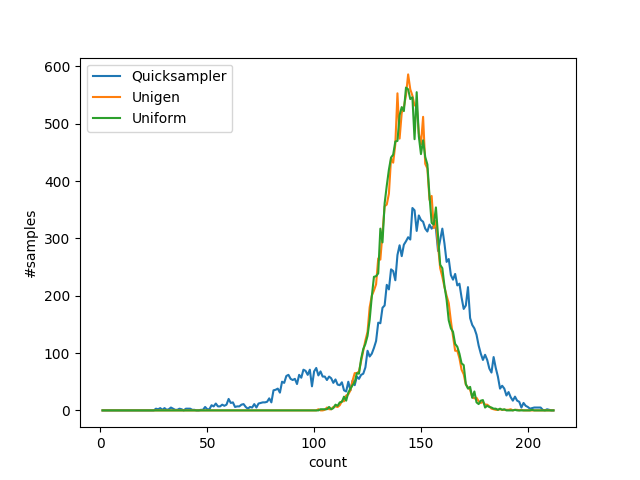
\includegraphics[scale=0.7]{DistributionFigures/Figure_case_110.png}
    \caption{blasted case 110}
\end{figure}
\begin{figure}[!h]
    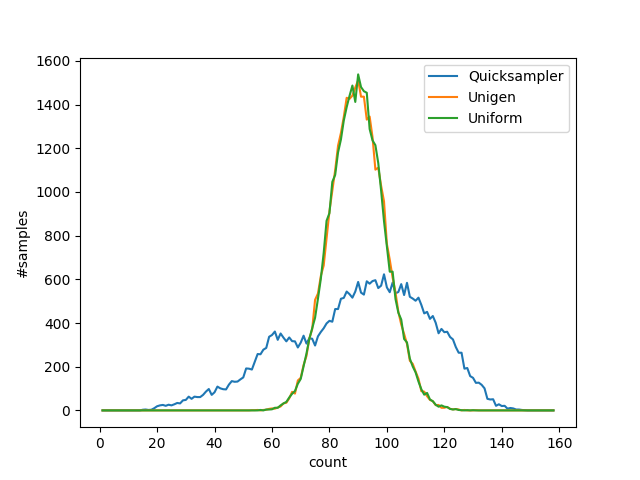
\includegraphics[scale=0.7]{DistributionFigures/Figure_case_59.png}
    \caption{blasted case 59}
\end{figure}
\begin{figure}[!h]
    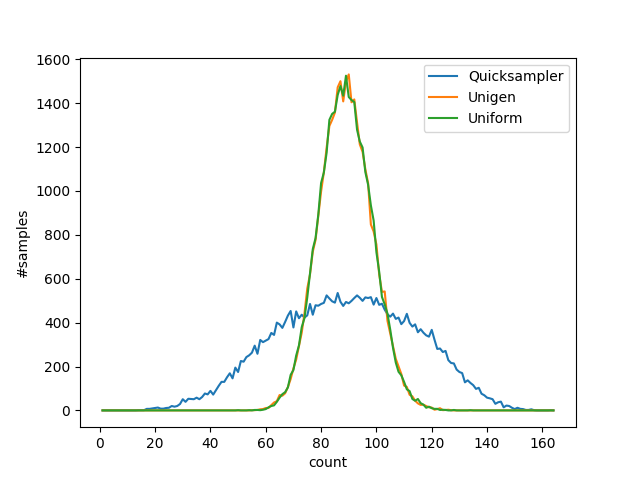
\includegraphics[scale=0.7]{DistributionFigures/Figure_case_59_1.png}
    \caption{blasted case 59.1}
\end{figure}
\begin{figure}[!h]
    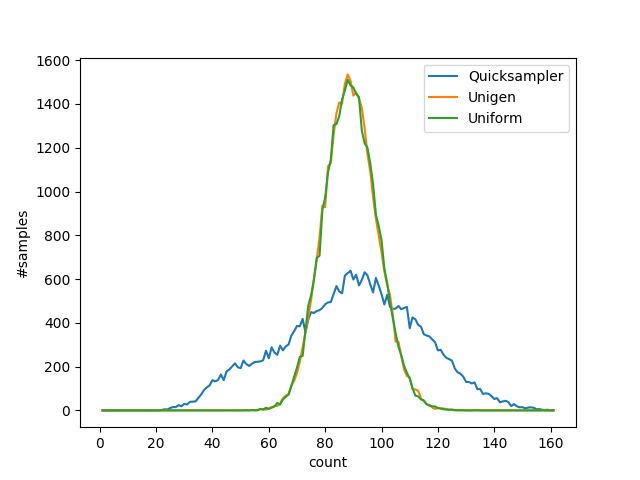
\includegraphics[scale=0.7]{DistributionFigures/Figure_case_64.png}
    \caption{blasted case 64}
\end{figure}
\begin{figure}[!h]
    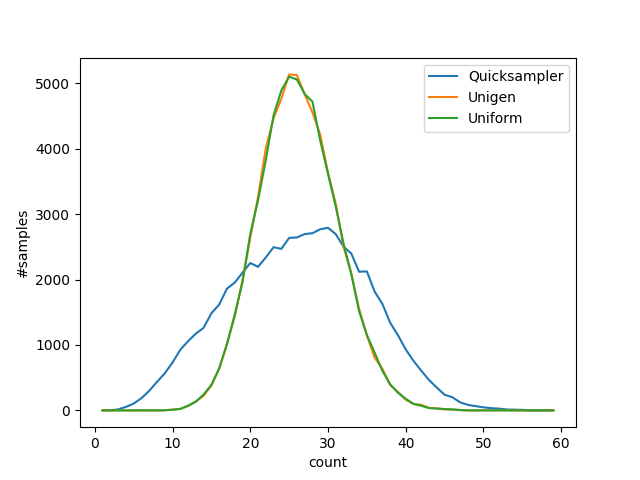
\includegraphics[scale=0.7]{DistributionFigures/Figure_s298.png}
    \caption{s298}
\end{figure}
\begin{figure}[!h]
    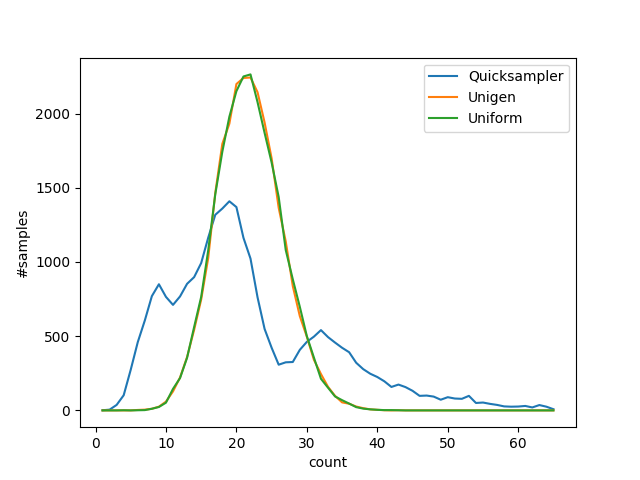
\includegraphics[scale=0.7]{DistributionFigures/Figure_JHipster.png}
    \caption{JHipster}
\end{figure}

\clearpage

\section{Impact du subsampling}

On trace la courbe de distribution de la formule \texttt{blasted\_case\_110} pour différents paramètres de subsampling. Initialement 5 milions de samples sont tirés. On en tire des sous échantillons aléatoirement parmi ces solutions, de tailles successives 2 millions, 1 million, 500'000, 200'000 et 100'000. On compare les figures de distribution obtenues.

\begin{figure}[!h]
    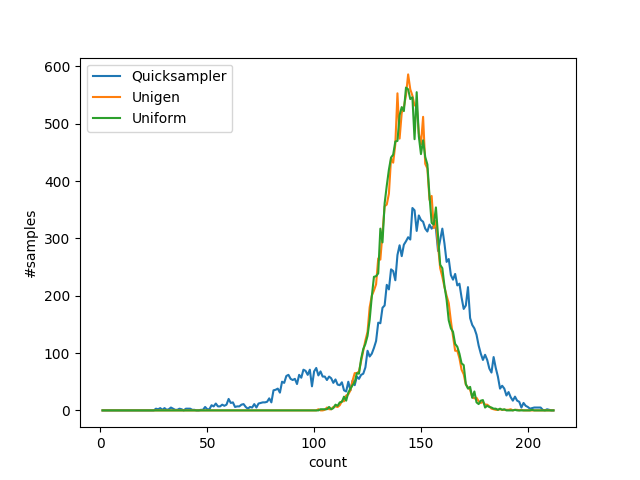
\includegraphics[scale=0.7]{DistributionFigures/Figure_case_110.png}
    \caption{Pas de sous-echantillonage}
\end{figure}
\begin{figure}[!h]
    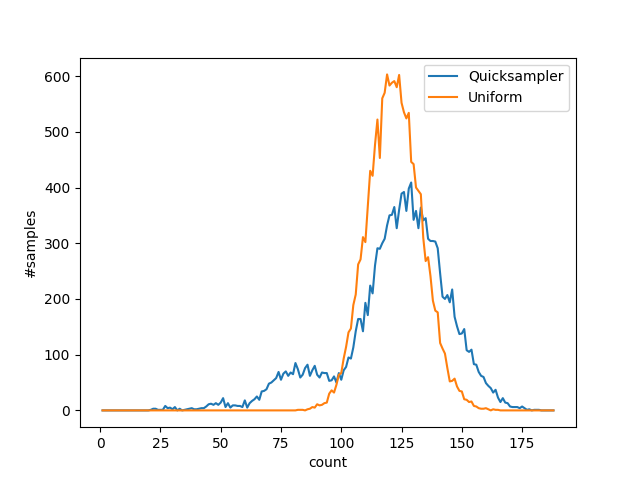
\includegraphics[scale=0.7]{DistributionFigures/Figure_case_110_2M.png}
    \caption{2 millions de sous-échantillons}
\end{figure}
\begin{figure}[!h]
    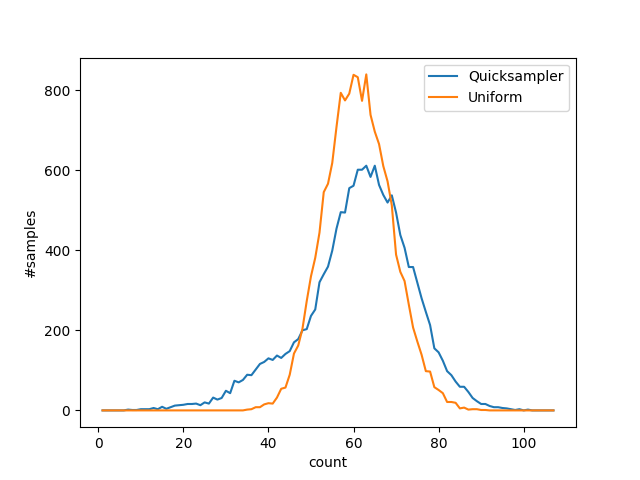
\includegraphics[scale=0.7]{DistributionFigures/Figure_case_110_1M.png}
    \caption{1 million de sous-échatillons}
\end{figure}
\begin{figure}[!h]
    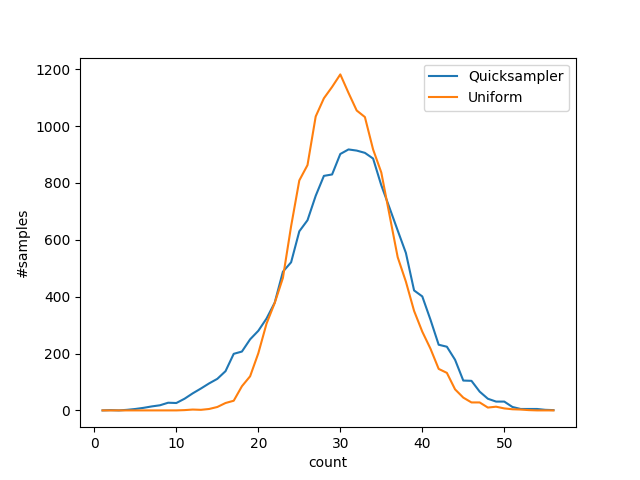
\includegraphics[scale=0.7]{DistributionFigures/Figure_case_110_500K.png}
    \caption{500'000 sous-échatillons}
\end{figure}
\begin{figure}[!h]
    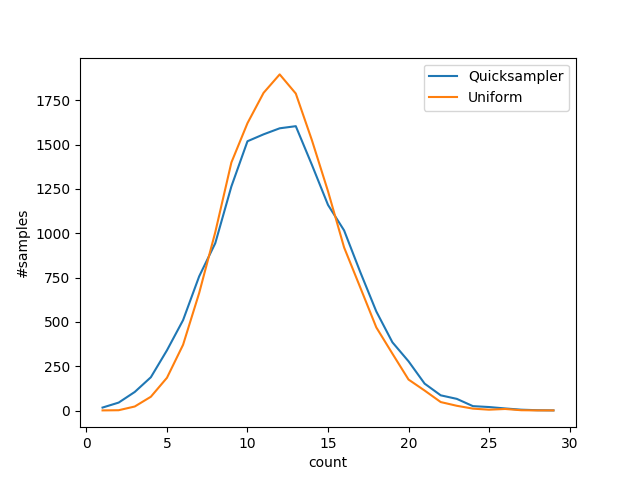
\includegraphics[scale=0.7]{DistributionFigures/Figure_case_110_200K.png}
    \caption{200'000 sous-échatillons}
\end{figure}
\begin{figure}[!h]
    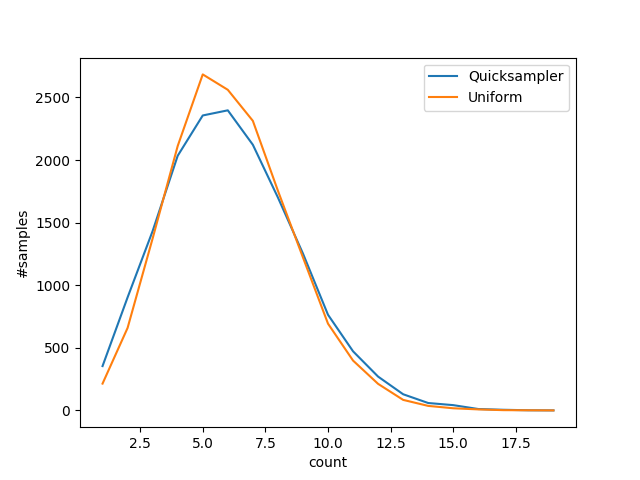
\includegraphics[scale=0.7]{DistributionFigures/Figure_case_110_100K.png}
    \caption{100'000 sous-échatillons}
\end{figure}

\clearpage

\section{Feature Models}

\hspace{-3cm}
\resizebox{18cm}{!}{
\begin{tabular}{|l r r r r| r r r r r r | r r|}
\hline
Benchmark & $|V|$ & Vars & Clauses & Solutions & $n$ & Calls & Samples & valid & $t_q (\mu s)$ & $t_q* (\mu s)$ & Samples & $t_u/t_q$ \\
\hline
aki3068net & 0.0 & 1207.0 & 3080.0 & 3.14854e121 & 0.0 & 34.0 & 516551.0 & 0.655 & 36.9 & 1234.8 & 0.0 & 0.0 \\
\hline
pc\_vmWare & 0.0 & 1255.0 & 3174.0 & 2.94320e126 & 0.0 & 36.0 & 505002.0 & 0.685 & 35.7 & 1255.2 & 0.0 & 0.0 \\
\hline
sleb & 0.0 & 1188.0 & 3009.0 & 1.19396e120 & 0.0 & 34.0 & 502533.0 & 0.663 & 33.6 & 1154.8 & 0.0 & 0.0 \\
\hline
eb55 & 0.0 & 1270.0 & 3882.0 & 3.01734e125 & 0.0 & 39.0 & 609304.0 & 0.787 & 30.3 & 1084.2 & 0.0 & 0.0 \\
\hline
vads & 0.0 & 1240.0 & 3235.0 & 2.91218e126 & 0.0 & 36.0 & 553838.0 & 0.663 & 35.5 & 1325.0 & 0.0 & 0.0 \\
\hline
ref4955 & 0.0 & 1218.0 & 3099.0 & 8.20319e123 & 0.0 & 37.0 & 518335.0 & 0.869 & 26.0 & 955.3 & 0.0 & 0.0 \\
\hline
se7751 & 0.0 & 1295.0 & 3254.0 & 1.11758e132 & 0.0 & 35.0 & 518230.0 & 0.602 & 40.5 & 1442.2 & 0.0 & 0.0 \\
\hline
aaed2000 & 0.0 & 1284.0 & 50512.0 & 2.82540e133 & 0.0 & 37.0 & 574346.0 & 0.608 & 45.9 & 2764.0 & 0.0 & 0.0 \\
\hline
iq80310 & 0.0 & 1258.0 & 3821.0 & 4.98043e127 & 0.0 & 39.0 & 598235.0 & 0.79 & 28.9 & 1129.4 & 0.0 & 0.0 \\
\hline
brutus & 0.0 & 1221.0 & 3754.0 & 1.47716e122 & 0.0 & 38.0 & 506587.0 & 0.804 & 30.8 & 1082.8 & 0.0 & 0.0 \\
\hline
pc\_rltk8139 & 0.0 & 1257.0 & 3179.0 & 6.88288e127 & 0.0 & 37.0 & 550904.0 & 0.792 & 31.5 & 1148.7 & 0.0 & 0.0 \\
\hline
mb93093 & 0.0 & 1230.0 & 3083.0 & 4.33253e129 & 0.0 & 37.0 & 520400.0 & 0.86 & 27.9 & 1016.6 & 0.0 & 0.0 \\
\hline
npwr & 0.0 & 1258.0 & 3822.0 & 1.25479e127 & 0.0 & 37.0 & 526926.0 & 0.705 & 33.1 & 1210.3 & 0.0 & 0.0 \\
\hline
olpcl2294 & 0.0 & 1273.0 & 3878.0 & 2.01769e127 & 0.0 & 36.0 & 506212.0 & 0.568 & 41.1 & 1480.1 & 0.0 & 0.0 \\
\hline
h8s\_sim & 0.0 & 1183.0 & 3003.0 & 1.26024e119 & 0.0 & 35.0 & 586233.0 & 0.674 & 31.8 & 1094.7 & 0.0 & 0.0 \\
\hline
pid & 0.0 & 1229.0 & 3778.0 & 1.03122e124 & 0.0 & 37.0 & 554645.0 & 0.649 & 35.2 & 1233.2 & 0.0 & 0.0 \\
\hline
am31\_sim & 0.0 & 1165.0 & 2968.0 & 3.15061e118 & 0.0 & 35.0 & 586386.0 & 0.712 & 29.6 & 1061.3 & 0.0 & 0.0 \\
\hline
nano & 0.0 & 1265.0 & 3870.0 & 5.03042e127 & 0.0 & 38.0 & 517977.0 & 0.728 & 31.9 & 1176.6 & 0.0 & 0.0 \\
\hline
grg & 0.0 & 1241.0 & 3792.0 & 1.41943e126 & 0.0 & 39.0 & 568628.0 & 0.788 & 28.7 & 1073.6 & 0.0 & 0.0 \\
\hline
eb40 & 0.0 & 1240.0 & 3816.0 & 2.51479e124 & 0.0 & 39.0 & 572203.0 & 0.824 & 27.5 & 1006.4 & 0.0 & 0.0 \\
\hline
asb & 0.0 & 1231.0 & 3081.0 & 2.08624e128 & 0.0 & 38.0 & 584896.0 & 0.779 & 28.3 & 1054.9 & 0.0 & 0.0 \\
\hline
uE250 & 0.0 & 1249.0 & 3810.0 & 2.94243e125 & 0.0 & 39.0 & 577611.0 & 0.767 & 30.0 & 1082.3 & 0.0 & 0.0 \\
\hline
sh7708 & 0.0 & 1253.0 & 49851.0 & 4.27966e122 & 0.0 & 36.0 & 543331.0 & 0.747 & 36.3 & 2152.6 & 0.0 & 0.0 \\
\hline
flexanet & 0.0 & 1265.0 & 3883.0 & 3.27890e126 & 0.0 & 37.0 & 559226.0 & 0.55 & 42.5 & 1519.1 & 0.0 & 0.0 \\
\hline
csb281 & 0.0 & 1233.0 & 3114.0 & 4.09125e125 & 0.0 & 37.0 & 538470.0 & 0.702 & 32.2 & 1178.8 & 0.0 & 0.0 \\
\hline
ceb\_v850 & 0.0 & 1189.0 & 3025.0 & 6.25341e120 & 0.0 & 36.0 & 568627.0 & 0.686 & 32.0 & 1134.9 & 0.0 & 0.0 \\
\hline
cerfpda & 0.0 & 1291.0 & 3940.0 & 2.56547e128 & 0.0 & 39.0 & 561925.0 & 0.804 & 29.5 & 1086.3 & 0.0 & 0.0 \\
\hline
malta\_mips64\_5kc & 0.0 & 1232.0 & 3212.0 & 1.80943e126 & 0.0 & 35.0 & 524171.0 & 0.733 & 31.6 & 1196.3 & 0.0 & 0.0 \\
\hline
viper & 0.0 & 1301.0 & 3230.0 & 5.79106e133 & 0.0 & 37.0 & 553736.0 & 0.707 & 33.9 & 1303.6 & 0.0 & 0.0 \\
\hline
pc\_i82559 & 0.0 & 1259.0 & 3179.0 & 1.83678e127 & 0.0 & 37.0 & 557931.0 & 0.714 & 32.6 & 1191.4 & 0.0 & 0.0 \\
\hline
lpcmt & 0.0 & 1249.0 & 3824.0 & 3.71280e124 & 0.0 & 37.0 & 577051.0 & 0.693 & 32.7 & 1194.7 & 0.0 & 0.0 \\
\hline
stm3210e\_eval & 0.0 & 1269.0 & 3200.0 & 4.91275e123 & 0.0 & 35.0 & 615453.0 & 0.669 & 33.9 & 1282.4 & 0.0 & 0.0 \\
\hline
frv400 & 0.0 & 1238.0 & 3096.0 & 3.49117e130 & 0.0 & 37.0 & 601077.0 & 0.811 & 26.9 & 1035.6 & 0.0 & 0.0 \\
\hline
pati & 0.0 & 1248.0 & 3266.0 & 7.90150e126 & 0.0 & 41.0 & 543809.0 & 0.879 & 26.8 & 1019.4 & 0.0 & 0.0 \\
\hline
ea2468 & 0.0 & 1395.0 & 4138.0 & 5.92126e130 & 0.0 & 40.0 & 592094.0 & 0.712 & 35.9 & 1295.0 & 0.0 & 0.0 \\
\hline
mb93091 & 0.0 & 1250.0 & 3131.0 & 1.68738e131 & 0.0 & 37.0 & 622184.0 & 0.781 & 27.6 & 1078.3 & 0.0 & 0.0 \\
\hline
excalibur\_arm9 & 0.0 & 1233.0 & 50538.0 & 1.91502e124 & 0.0 & 38.0 & 566744.0 & 0.731 & 35.3 & 2220.7 & 0.0 & 0.0 \\
\hline
linux & 0.0 & 1232.0 & 3154.0 & 1.13408e122 & 0.0 & 35.0 & 605514.0 & 0.597 & 37.4 & 1349.5 & 0.0 & 0.0 \\
\hline
gps4020 & 0.0 & 1213.0 & 3743.0 & 1.76978e122 & 0.0 & 36.0 & 510253.0 & 0.604 & 36.8 & 1286.7 & 0.0 & 0.0 \\
\hline
cme555 & 0.0 & 1266.0 & 3167.0 & 1.32433e133 & 0.0 & 39.0 & 509158.0 & 0.698 & 34.7 & 1243.7 & 0.0 & 0.0 \\
\hline
sam7ex256 & 0.0 & 1332.0 & 3989.0 & 9.44851e131 & 0.0 & 38.0 & 613766.0 & 0.649 & 36.3 & 1387.9 & 0.0 & 0.0 \\
\hline
vrc4375 & 0.0 & 1258.0 & 3129.0 & 3.30843e133 & 0.0 & 35.0 & 501572.0 & 0.728 & 32.4 & 1280.6 & 0.0 & 0.0 \\
\hline
sa1100mm & 0.0 & 1222.0 & 3760.0 & 2.09616e122 & 0.0 & 38.0 & 521726.0 & 0.753 & 35.2 & 1241.9 & 0.0 & 0.0 \\
\hline
sparc\_erc32 & 0.0 & 1168.0 & 2972.0 & 3.15061e118 & 0.0 & 34.0 & 606018.0 & 0.558 & 45.4 & 1612.7 & 0.0 & 0.0 \\
\hline
phycore229x & 0.0 & 1360.0 & 4026.0 & 1.76902e136 & 0.0 & 39.0 & 513660.0 & 0.728 & 42.6 & 1511.7 & 0.0 & 0.0 \\
\hline
ipaq & 0.0 & 1258.0 & 3868.0 & 3.32881e123 & 0.0 & 38.0 & 575738.0 & 0.766 & 35.7 & 1292.8 & 0.0 & 0.0 \\
\hline
snds & 0.0 & 1218.0 & 3748.0 & 2.13275e123 & 0.0 & 35.0 & 504228.0 & 0.526 & 54.0 & 1763.6 & 0.0 & 0.0 \\
\hline
fads & 0.0 & 1187.0 & 3008.0 & 2.24981e121 & 0.0 & 37.0 & 514802.0 & 0.766 & 29.4 & 1008.9 & 0.0 & 0.0 \\
\hline
olpce2294 & 0.0 & 1274.0 & 3881.0 & 8.18796e126 & 0.0 & 37.0 & 596183.0 & 0.654 & 43.5 & 1792.3 & 0.0 & 0.0 \\
\hline
edb7xxx & 0.0 & 1246.0 & 3812.0 & 4.78426e125 & 0.0 & 37.0 & 605852.0 & 0.646 & 48.1 & 1801.2 & 0.0 & 0.0 \\
\hline
cerf & 0.0 & 1276.0 & 3910.0 & 1.35173e127 & 0.0 & 38.0 & 509585.0 & 0.692 & 37.9 & 1449.4 & 0.0 & 0.0 \\
\hline
pc\_usb\_d12 & 0.0 & 1281.0 & 3231.0 & 7.24452e128 & 0.0 & 37.0 & 603130.0 & 0.732 & 39.5 & 1446.4 & 0.0 & 0.0 \\
\hline
rattler & 0.0 & 1311.0 & 3245.0 & 3.63416e136 & 0.0 & 37.0 & 581475.0 & 0.699 & 42.5 & 1470.2 & 0.0 & 0.0 \\
\hline
ocelot & 0.0 & 1266.0 & 3141.0 & 1.22441e134 & 0.0 & 34.0 & 514910.0 & 0.632 & 40.7 & 1465.8 & 0.0 & 0.0 \\
\hline
sparc\_leon & 0.0 & 1168.0 & 2972.0 & 3.15061e118 & 0.0 & 34.0 & 513543.0 & 0.619 & 37.4 & 1265.0 & 0.0 & 0.0 \\
\hline
h8max & 0.0 & 1202.0 & 3072.0 & 1.05885e121 & 0.0 & 35.0 & 549890.0 & 0.683 & 35.0 & 1197.6 & 0.0 & 0.0 \\
\hline
calm16\_ceb & 0.0 & 1173.0 & 2990.0 & 7.76740e118 & 0.0 & 34.0 & 568229.0 & 0.592 & 40.7 & 1442.7 & 0.0 & 0.0 \\
\hline
eb42 & 0.0 & 1234.0 & 3779.0 & 1.07789e124 & 0.0 & 39.0 & 558709.0 & 0.851 & 30.0 & 1110.0 & 0.0 & 0.0 \\
\hline
atlas\_mips64\_5kc & 0.0 & 1209.0 & 3066.0 & 1.20547e123 & 0.0 & 35.0 & 538049.0 & 0.735 & 34.5 & 1251.4 & 0.0 & 0.0 \\
\hline
skmb91302 & 0.0 & 1217.0 & 3052.0 & 1.04312e128 & 0.0 & 38.0 & 613275.0 & 0.883 & 29.8 & 1093.6 & 0.0 & 0.0 \\
\hline
mace1 & 0.0 & 1234.0 & 3770.0 & 6.56138e122 & 0.0 & 36.0 & 505954.0 & 0.631 & 44.0 & 1500.7 & 0.0 & 0.0 \\
\hline
asb2305 & 0.0 & 1242.0 & 3101.0 & 4.17249e128 & 0.0 & 35.0 & 513198.0 & 0.593 & 45.9 & 1618.0 & 0.0 & 0.0 \\
\hline
hs7729pci & 0.0 & 1298.0 & 49911.0 & 3.31375e132 & 0.0 & 36.0 & 517514.0 & 0.732 & 46.7 & 2860.2 & 0.0 & 0.0 \\
\hline
e7t & 0.0 & 1266.0 & 3816.0 & 1.19421e134 & 0.0 & 36.0 & 518381.0 & 0.561 & 51.0 & 1854.4 & 0.0 & 0.0 \\
\hline
phycore & 0.0 & 1274.0 & 3852.0 & 3.23967e133 & 0.0 & 37.0 & 576664.0 & 0.665 & 44.8 & 1675.3 & 0.0 & 0.0 \\
\hline
innovator & 0.0 & 1256.0 & 50452.0 & 2.27314e132 & 0.0 & 37.0 & 625146.0 & 0.634 & 50.5 & 3581.2 & 0.0 & 0.0 \\
\hline
aeb & 0.0 & 1213.0 & 3767.0 & 6.21586e121 & 0.0 & 37.0 & 517002.0 & 0.736 & 30.6 & 1088.7 & 0.0 & 0.0 \\
\hline
h8300h\_sim & 0.0 & 1182.0 & 3001.0 & 1.26024e119 & 0.0 & 35.0 & 539056.0 & 0.685 & 31.2 & 1113.9 & 0.0 & 0.0 \\
\hline
adder & 0.0 & 1272.0 & 3201.0 & 9.88262e124 & 0.0 & 37.0 & 604929.0 & 0.648 & 34.4 & 1301.1 & 0.0 & 0.0 \\
\hline
cq7750 & 0.0 & 1267.0 & 3173.0 & 2.51812e129 & 0.0 & 36.0 & 587374.0 & 0.721 & 31.8 & 1132.8 & 0.0 & 0.0 \\
\hline
ixdp425 & 0.0 & 1247.0 & 3799.0 & 5.96186e126 & 0.0 & 37.0 & 558076.0 & 0.679 & 33.7 & 1196.5 & 0.0 & 0.0 \\
\hline
mbx & 0.0 & 1295.0 & 3218.0 & 3.08602e133 & 0.0 & 38.0 & 566315.0 & 0.779 & 30.1 & 1149.1 & 0.0 & 0.0 \\
\hline
ts6 & 0.0 & 1240.0 & 3235.0 & 2.91218e126 & 0.0 & 36.0 & 512390.0 & 0.754 & 30.1 & 1143.4 & 0.0 & 0.0 \\
\hline
se77x9 & 0.0 & 1319.0 & 49937.0 & 1.20026e135 & 0.0 & 37.0 & 598315.0 & 0.783 & 35.0 & 2258.0 & 0.0 & 0.0 \\
\hline
eb40a & 0.0 & 1241.0 & 3817.0 & 2.51479e124 & 0.0 & 37.0 & 527173.0 & 0.719 & 32.0 & 1138.3 & 0.0 & 0.0 \\
\hline
moab & 0.0 & 1277.0 & 3249.0 & 3.79666e128 & 0.0 & 36.0 & 516367.0 & 0.731 & 32.3 & 1201.6 & 0.0 & 0.0 \\
\hline
cma28x & 0.0 & 1204.0 & 3051.0 & 2.37571e122 & 0.0 & 37.0 & 608789.0 & 0.674 & 32.6 & 1149.2 & 0.0 & 0.0 \\
\hline
cma230 & 0.0 & 1212.0 & 3739.0 & 6.40768e121 & 0.0 & 37.0 & 554404.0 & 0.699 & 32.1 & 1124.3 & 0.0 & 0.0 \\
\hline
assabet & 0.0 & 1266.0 & 3883.0 & 1.52853e125 & 0.0 & 39.0 & 612050.0 & 0.811 & 29.3 & 1053.8 & 0.0 & 0.0 \\
\hline
cq7708 & 0.0 & 1238.0 & 49770.0 & 5.16325e121 & 0.0 & 35.0 & 593795.0 & 0.546 & 44.9 & 2696.4 & 0.0 & 0.0 \\
\hline
jtst & 0.0 & 1241.0 & 3818.0 & 1.51214e124 & 0.0 & 37.0 & 511750.0 & 0.761 & 29.8 & 1068.9 & 0.0 & 0.0 \\
\hline
edosk2674 & 0.0 & 1194.0 & 3034.0 & 2.73597e120 & 0.0 & 34.0 & 501301.0 & 0.658 & 33.4 & 1168.2 & 0.0 & 0.0 \\
\hline
mcb2100 & 0.0 & 1249.0 & 3824.0 & 3.71280e124 & 0.0 & 37.0 & 584895.0 & 0.675 & 33.8 & 1216.0 & 0.0 & 0.0 \\
\hline
FM-3.6.1-refined & 0.0 & 45.0 & 104.0 & 26256 & 7.0 & 311.0 & 504119.0 & 0.123 & 26.4 & 91.4 & 0.0 & 0.0 \\
\hline
jmr3904 & 0.0 & 1199.0 & 3035.0 & 4.73549e121 & 0.0 & 37.0 & 578337.0 & 0.847 & 24.8 & 919.1 & 0.0 & 0.0 \\
\hline
sh4\_202\_md & 0.0 & 1258.0 & 3196.0 & 1.83198e123 & 0.0 & 36.0 & 603814.0 & 0.703 & 33.6 & 1162.7 & 0.0 & 0.0 \\
\hline
ts1000 & 0.0 & 1297.0 & 3218.0 & 1.18361e134 & 0.0 & 39.0 & 583926.0 & 0.79 & 29.1 & 1116.6 & 0.0 & 0.0 \\
\hline
mpc50 & 0.0 & 1213.0 & 3728.0 & 3.16818e122 & 0.0 & 39.0 & 549172.0 & 0.823 & 26.9 & 980.0 & 0.0 & 0.0 \\
\hline
integrator\_arm7 & 0.0 & 1259.0 & 3939.0 & 9.01857e128 & 0.0 & 39.0 & 505129.0 & 0.814 & 29.5 & 1083.8 & 0.0 & 0.0 \\
\hline
pc\_i82544 & 0.0 & 1259.0 & 3179.0 & 1.83678e127 & 0.0 & 37.0 & 586327.0 & 0.767 & 29.8 & 1093.5 & 0.0 & 0.0 \\
\hline
tx39\_sim & 0.0 & 1179.0 & 2988.0 & 6.82632e119 & 0.0 & 37.0 & 614433.0 & 0.797 & 26.5 & 1035.7 & 0.0 & 0.0 \\
\hline
at91sam7xek & 0.0 & 1319.0 & 3963.0 & 9.44851e131 & 0.0 & 39.0 & 577177.0 & 0.821 & 29.3 & 1124.9 & 0.0 & 0.0 \\
\hline
mac7100evb & 0.0 & 1234.0 & 3770.0 & 6.56138e122 & 0.0 & 37.0 & 525868.0 & 0.769 & 28.9 & 1052.6 & 0.0 & 0.0 \\
\hline
psim & 0.0 & 1181.0 & 2995.0 & 1.34531e121 & 0.0 & 38.0 & 526961.0 & 0.857 & 24.6 & 916.3 & 0.0 & 0.0 \\
\hline
refidt334 & 0.0 & 1263.0 & 3140.0 & 2.94575e134 & 0.0 & 35.0 & 559277.0 & 0.671 & 33.7 & 1285.8 & 0.0 & 0.0 \\
\hline
smdk2410 & 0.0 & 1265.0 & 50468.0 & 2.23804e131 & 0.0 & 37.0 & 548287.0 & 0.7 & 37.8 & 2519.7 & 0.0 & 0.0 \\
\hline
stb & 0.0 & 1252.0 & 3146.0 & 6.67873e129 & 0.0 & 38.0 & 564589.0 & 0.817 & 26.9 & 1035.6 & 0.0 & 0.0 \\
\hline
atlas\_mips32\_4kc & 0.0 & 1216.0 & 3078.0 & 3.01370e123 & 0.0 & 35.0 & 522534.0 & 0.756 & 29.6 & 1067.3 & 0.0 & 0.0 \\
\hline
sparclite\_sim & 0.0 & 1168.0 & 2972.0 & 3.15061e118 & 0.0 & 34.0 & 545468.0 & 0.606 & 35.2 & 1216.1 & 0.0 & 0.0 \\
\hline
iq80321 & 0.0 & 1256.0 & 3820.0 & 2.53426e127 & 0.0 & 37.0 & 595140.0 & 0.695 & 32.8 & 1223.0 & 0.0 & 0.0 \\
\hline
ebsa285 & 0.0 & 1245.0 & 3832.0 & 3.68860e126 & 0.0 & 37.0 & 563306.0 & 0.634 & 36.3 & 1357.5 & 0.0 & 0.0 \\
\hline
adderII & 0.0 & 1276.0 & 3206.0 & 3.57233e125 & 0.0 & 37.0 & 558117.0 & 0.708 & 32.1 & 1241.6 & 0.0 & 0.0 \\
\hline
at91sam7sek & 0.0 & 1296.0 & 3921.0 & 2.58921e127 & 0.0 & 39.0 & 595149.0 & 0.786 & 28.9 & 1094.4 & 0.0 & 0.0 \\
\hline
calm32\_ceb & 0.0 & 1173.0 & 2990.0 & 7.76740e118 & 0.0 & 35.0 & 500032.0 & 0.797 & 26.5 & 951.1 & 0.0 & 0.0 \\
\hline
malta\_mips32\_4kc & 0.0 & 1232.0 & 3213.0 & 9.04717e125 & 0.0 & 39.0 & 613844.0 & 0.915 & 23.2 & 990.3 & 0.0 & 0.0 \\
\hline
prpmc1100 & 0.0 & 1223.0 & 3754.0 & 2.38677e123 & 0.0 & 37.0 & 537632.0 & 0.719 & 31.1 & 1095.0 & 0.0 & 0.0 \\
\hline
vrc4373 & 0.0 & 1247.0 & 3104.0 & 5.09202e131 & 0.0 & 34.0 & 535147.0 & 0.525 & 43.8 & 1567.7 & 0.0 & 0.0 \\
\hline
olpch2294 & 0.0 & 1261.0 & 3851.0 & 1.95289e125 & 0.0 & 38.0 & 579837.0 & 0.772 & 29.3 & 1065.0 & 0.0 & 0.0 \\
\hline
picasso & 0.0 & 1248.0 & 3808.0 & 1.80467e125 & 0.0 & 36.0 & 512385.0 & 0.65 & 35.0 & 1265.7 & 0.0 & 0.0 \\
\hline
ec555 & 0.0 & 1267.0 & 3169.0 & 1.32433e133 & 0.0 & 41.0 & 501396.0 & 0.768 & 30.6 & 1119.0 & 0.0 & 0.0 \\
\hline
stdeval1 & 0.0 & 1190.0 & 3049.0 & 2.16555e120 & 0.0 & 37.0 & 576792.0 & 0.814 & 25.8 & 991.4 & 0.0 & 0.0 \\
\hline
m5272c3 & 0.0 & 1323.0 & 3297.0 & 2.36757e125 & 0.0 & 36.0 & 560636.0 & 0.675 & 36.2 & 1317.6 & 0.0 & 0.0 \\
\hline
dreamcast & 0.0 & 1252.0 & 3168.0 & 1.09233e123 & 0.0 & 36.0 & 581903.0 & 0.752 & 30.8 & 1109.8 & 0.0 & 0.0 \\
\hline
XSEngine & 0.0 & 1260.0 & 3803.0 & 2.04657e133 & 0.0 & 37.0 & 571987.0 & 0.641 & 35.5 & 1286.1 & 0.0 & 0.0 \\
\hline
aim711 & 0.0 & 1264.0 & 3873.0 & 1.82286e127 & 0.0 & 41.0 & 611650.0 & 0.936 & 23.9 & 936.6 & 0.0 & 0.0 \\
\hline
p2106 & 0.0 & 1249.0 & 3824.0 & 3.71280e124 & 0.0 & 38.0 & 595044.0 & 0.756 & 30.0 & 1106.8 & 0.0 & 0.0 \\
\hline
integrator\_arm9 & 0.0 & 1267.0 & 50606.0 & 4.05835e129 & 0.0 & 41.0 & 617111.0 & 0.821 & 31.5 & 2054.4 & 0.0 & 0.0 \\
\hline
uClinux-config & 0.0 & 11254.0 & 31637.0 & 7.78028e417 & 0.0 & 64.0 & 1149017.0 & 1.0 & 157.0 & 11948.2 & 0.0 & 0.0 \\
\hline
toybox & 68.0 & 544.0 & 1020.0 & 1.44991e17 & 0.0 & 37.0 & 1075381.0 & 0.898 & 3.6 & 59.7 & 0.0 & 0.0 \\
\hline
\end{tabular}
}

\section{FMEasy}

\hspace{-3cm}
\resizebox{18cm}{!}{
\begin{tabular}{|l r r r r| r r r r r r | r r|}
\hline
Benchmark & $|V|$ & Vars & Clauses & Solutions & $n$ & Calls & Samples & valid & $t_q (\mu s)$ & $t_q* (\mu s)$ & Samples & $t_u/t_q$ \\
\hline
uClinux-config & 0.0 & 11254.0 & 31637.0 & 7.78028e417 & 0.0 & 64.0 & 1149017.0 & 1.0 & 193.5 & 11548.7 & 0.0 & 0.0 \\
\hline
toybox & 68.0 & 544.0 & 1020.0 & 1.44991e17 & 0.0 & 36.0 & 1021556.0 & 0.895 & 3.7 & 59.3 & 0.0 & 0.0 \\
\hline
embtoolkit & 0.0 & 0.0 & 0.0 &  0 & 0.0 & 0.0 & 0.0 & 0.0 & 0.0 & 0.0 & 0.0 & 0.0 \\
\hline
coreboot & 0.0 & 12268.0 & 47091.0 & 1.40174e94 & 0.0 & 80.0 & 1149017.0 & 0.144 & 2640.0 & 30019.9 & 0.0 & 0.0 \\
\hline
busybox-1.18.0 & 0.0 & 6796.0 & 17836.0 & 8.49902e216 & 0.0 & 64.0 & 1149017.0 & 0.725 & 113.2 & 5098.2 & 0.0 & 0.0 \\
\hline
axTLS & 0.0 & 684.0 & 2155.0 & 4.28726e20 & 0.0 & 70.0 & 1098865.0 & 0.386 & 30.1 & 581.9 & 0.0 & 0.0 \\
\hline
2.6.28.6-icse11 & 0.0 & 6888.0 & 343944.0 & nan & 0.0 & 33.0 & 1089245.0 & 0.13 & 1124.9 & 31766.0 & 0.0 & 0.0 \\
\hline
fiasco & 0.0 & 1638.0 & 5228.0 & 3.58108e14 & 0.0 & 86.0 & 1080270.0 & 0.047 & 639.1 & 9715.6 & 0.0 & 0.0 \\
\hline
uClinux & 0.0 & 1850.0 & 2468.0 & 1.62962e91 & 0.0 & 64.0 & 1149017.0 & 1.0 & 21.3 & 358.9 & 0.0 & 0.0 \\
\hline
freetz & 0.0 & 31012.0 & 102705.0 & nan & 0.0 & 0.0 & 1.0 & 43316.0 & 83110.2 & 183603.2 & 0.0 & 0.0 \\
\hline
toybox2 & 68.0 & 544.0 & 1020.0 & 1.44991e17 & 0.0 & 37.0 & 1129007.0 & 0.892 & 3.6 & 59.2 & 0.0 & 0.0 \\
\hline
buildroot & 0.0 & 14910.0 & 45603.0 & nan & 0.0 & 64.0 & 1085562.0 & 0.14 & 2619.5 & 31226.5 & 0.0 & 0.0 \\
\hline
ecos-icse11 & 0.0 & 1244.0 & 3146.0 & 4.97468e125 & 0.0 & 63.0 & 1173038.0 & 0.816 & 24.6 & 987.5 & 0.0 & 0.0 \\
\hline
2.6.33.3-2var & 0.0 & 62482.0 & 273799.0 & nan & 0.0 & 0.0 & 1.0 & 0.0 & nan & nan & 0.0 & nan \\
\hline
freebsd-icse11 & 0.0 & 1396.0 & 62183.0 & 8.38866e313 & 0.0 & 35.0 & 1152001.0 & 0.402 & 75.6 & 8228.4 & 0.0 & 0.0 \\
\hline
2.6.32-2var & 0.0 & 60072.0 & 268223.0 & nan & 0.0 & 0.0 & 1.0 & 0.0 & nan & nan & 0.0 & nan \\
\hline
\end{tabular}
}

\end{document}
